% !TeX root = ../main.tex
\chapter{Examples from Industry}\label{chapter:examples}

This chapter gives an overview of the broad history of video streaming and then presents three aspects of video services in detail using examples from the well known video streaming services: First a look at the general system design and architecture of a streaming service, using the example of Twitch, then a look at how Netflix works together with \ac{ISPs} to deliver content as efficiently as possible, and lastly a section on how YouTube has handled different scalability challenges and developed its own warehouse-scale video transcoding system.     

\section{History}
The video streaming industry has evolved dramatically over the past decades, transitioning from old fashioned technologies to highly complex, scalable infrastructures capable of delivering large amounts of content to millions of users simultaneously. The origins of video streaming can be traced back to the late 1990s and early 2000s, with the introduction of streaming technologies like RealNetworks' RealPlayer and Apple's QuickTime. These early platforms allowed users to stream audio and video content, although at low quality and with significant buffering issues due to limited bandwidth and server capacities.
Another important precursor to modern streaming was \ac{MBone}, a virtual network introduced in the early 1990s to support audio and video broadcasts over the internet showing the potential behind internet-based multimedia transmission. 
Around 2002, the interest in a single, unified, streaming format and the widespread adoption of Adobe Flash started the development of a video streaming format through Flash which was the format used in Flash-based players on video hosting sites.
The real breakthrough in video streaming came in 2005 with the launch of YouTube, which introduced a user-friendly platform for uploading, sharing, and streaming videos online. YouTube's success not only showed the willingness of users to consume hours of uploaded video content via the internet, but also the potential for scalable video streaming infrastructure, increasing the demand for online video content. At the same time, Netflix's pivot from a mail-based DVD rental business to streaming in 2007 set another milestone in the industry. 

As internet speeds increased and cloud computing became more prevalent, the scalability of video streaming services improved. By August 2016, Netflix closed its last physical data center, but continued to develop its Open Connect technology~\parencite{netflix_cloud}.
Additionally, the introduction of \ac{ABR} streaming allowed platforms to dynamically adjust video quality based on the user's internet connection, reducing buffering and improving the overall viewing experience~\parencite{abr}. Meanwhile, \ac{CDN}s became a critical component of streaming infrastructure by caching video data closer to users, thereby reducing latency and server load~\parencite{cdn_basic}.

% \section{Statistics}
% TODO (?)
% As of 2024, video streaming accounts for over 82\% of all internet traffic, driven by the always increasing popularity of platforms like YouTube, Netflix, and ~\parencite{cisco_vni}. The global video streaming market, valued at approximately \$90 billion in 2023, is projected to grow to over \$150 billion by 2028~\parencite{grandview_research}. This growth is fueled by the demand for high-quality video content, including 4K and 8K resolutions, and the increasing availability of high-speed internet access worldwide.

% YouTube, the largest video-sharing platform, reported over 2 billion logged-in monthly users who watch over 1 billion hours of video daily~\parencite{youtube_stats}. The platform's user base generates immense amounts of data, requiring a highly scalable and efficient infrastructure to manage content delivery and storage. Twitch, the leading platform for live streaming, particularly in the gaming sector, currently has over 140 million unique monthly viewers. At any given time, there are approximately 2.5 million concurrent viewers on Twitch~\parencite{twitch_stats}.

% Also, the shift towards mobile video consumption is another significant trend, with over 60\% of video streams now being viewed on mobile devices~\parencite{mobile_video}. This trend has required further optimization of streaming infrastructure to account for the variability in mobile network conditions and the need for efficient data usage.

\section{Example: Twitch}
Twitch, which launched in 2011 as a spin-off from the general-interest streaming platform Justin.tv, has become synonymous with live streaming, particularly within the gaming community. Its popularity can be explained by its ability to deliver high-quality, low-latency streams to millions of users simultaneously. 
One of the most significant challenges Twitch faces is the need to manage vast amounts of user-generated content in real-time and scale with high fluctuations in viewer numbers, particularly during major events like e-sports competitions.
Twitch's architecture is highly complex and needs to support millions of concurrent video streams, real-time interactions through chat, and extensive data processing. In the following, there is a detailed breakdown of the key components of its architecture (see also \autoref{fig:twitch-architecture}):

\begin{figure}[htpb]
    \centering
    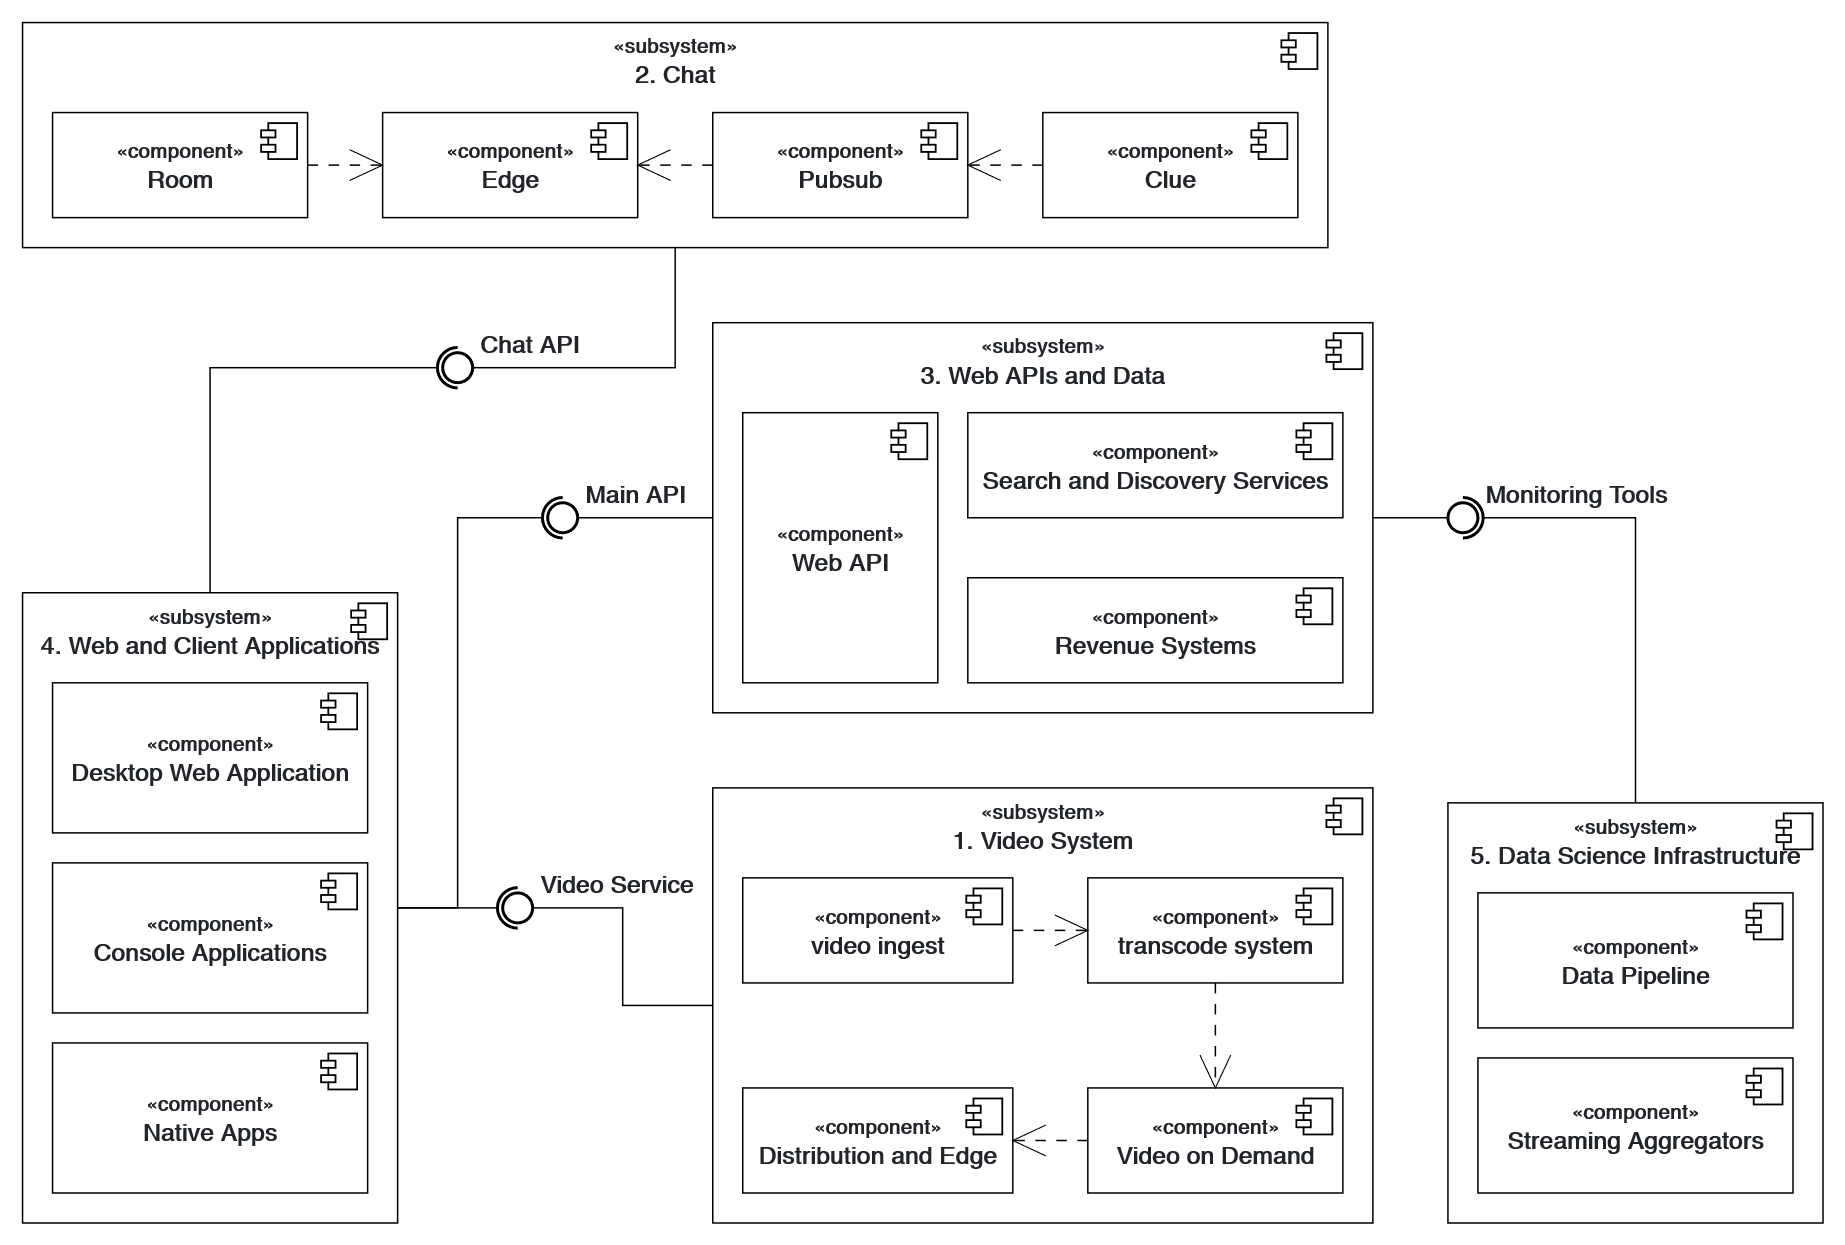
\includegraphics[width=\linewidth]{images/TwitchArchitecture.png}
    \caption[Twitch Architecture]{Twitch Architecture}\label{fig:twitch-architecture}
\end{figure}

\begin{enumerate}
    \item \textbf{Video System}
    
    The video system begins with the \textbf{video ingest} process, where live video streams are received from broadcasters. Twitch primarily uses \ac{RTMP} for this purpose. Once the video stream is ingested, it is transported to the \textbf{transcode system}. This system, implemented in a combination of C/C++ and Go, transcodes the incoming \ac{RTMP} stream into multiple \ac{HLS} streams to allow viewers to switch between different quality streams.
    After transcoding, the streams are distributed through Twitch's global \textbf{Distribution and Edge} network consisting of multiple \ac{POPs}. The \ac{POPs} cache the \ac{HLS} streams and deliver them to users from geographically optimal locations, minimizing latency and buffering. The distribution system, also largely written in Go, is designed to scale massively, ensuring high availability even during peak usage times. Additionally, Twitch archives all live streams through its \textbf{\ac{VOD} system}, making content available for later viewing, either immediately after the live broadcast or as part of a long-term archive~\parencite{twitch_engineering}.
    
    \item \textbf{Chat}

    The chat system is a real-time distributed system, primarily written in Go, and designed to handle real-time interaction between viewers and streamers. The \textbf{Edge} component of the chat system is responsible for receiving and distributing messages between clients and backend services. It supports the \ac{IRC} protocol over both raw TCP and WebSockets, which allows for broad compatibility, including the integration of third-party \ac{IRC} bots.
    
    Next, the \textbf{Pubsub} subsystem is used for the internal distribution of chat messages across various edge nodes. Together, they create a hierarchical message distribution system capable of executing massive fanout, ensuring that all participants in a chat room receive messages promptly and reliably. The \textbf{Clue} component handles the application of business logic to chat interactions. For instance, it checks if a user is banned from a channel, whether they are a subscriber, or if they are exhibiting abusive behavior. Clue achieves this by aggregating data from various sources, including databases, internal \ac{API}s, and caches, to make real-time decisions. Finally, the \textbf{Room} component manages the viewer list for each chat room. It aggregates, stores, and queries membership data across all Edge nodes to provide accurate and up-to-date viewer lists, which are crucial for both moderation and user interaction~\parencite{twitch_chat}.

    \item \textbf{Web \ac{API}s and Data}

    Twitch’s platform also includes a set of web \ac{API}s and data services that enable various functionalities, from user profile management to stream discovery. These \textbf{Web \ac{API}s} are built using a combination of Ruby on Rails, Go, and other open-source technologies, designed to handle high request volumes, with Twitch's services processing over 50,000 \ac{API} requests per second on average. These \ac{API}s allow users to manage their profiles, customize subscriptions, and interact with other services on the platform~\parencite{twitch_engineering}.

    Additionally, Twitch also has various micro services for specific use cases such as \textbf{Search and Discovery Services} to help users find streams and content that match their interests or \textbf{Revenue Systems} that manage all aspects of advertising and subscriptions, ensuring that revenue is accurately tracked and distributed to partners~\parencite{twitch_engineering}. 
    
    \item \textbf{Web and Client Applications}
    
    Twitch’s \textbf{Desktop Web Application} began as a vanilla Rails application but has developed into a Ember.js application. For mobile users, Twitch offers \textbf{Native Apps} on iOS and Android platforms as well as \textbf{Console Applications} for major gaming systems, including Xbox One, Xbox 360, and PlayStation 4~\parencite{twitch_engineering}.

    \item \textbf{Data Science Infrastructure}

    Next to its operating infrastructure, Twitch’s data science infrastructure plays an important role in optimizing the platform, improving user experiences, and driving business decisions. At the core of this infrastructure is the \textbf{Data Pipeline}, which is responsible for collecting, cleaning, and loading over a billion events per day into Twitch’s data warehouse~\parencite{twitch_engineering}. 

    The platform also uses so called \textbf{Streaming Aggregators}, which summarize key metrics in near real-time. These aggregators provide broadcasters with immediate feedback on their stream performance, allowing them to make adjustments on the fly to improve viewer engagement~\parencite{twitch_engineering}.

    \item \textbf{Tools and Operational Infrastructure}

    \ac{QA} is critical, with Twitch utilizing both \textbf{Automated Testing Frameworks} such as Jenkins to allow for continuous integration and testing to maintain high code quality across all services.

    In addition to that, there are also several \textbf{Deployment and Rollback Tools}, as well as \textbf{Monitoring and Alerting Systems}, including Ganglia, Graphite, and Nagios that monitor the health and performance of the infrastructure, providing real-time alerts and insights that help engineers quickly identify and prevent problems~\parencite{twitch_engineering}.

    Lastly, Twitch’s \textbf{Network Infrastructure} mostly operates on bare-metal \ac{POPs} worldwide while an increasing number of services are being migrated to \ac{AWS}, which helps reduce operational overhead while benefiting from the on-demand scalability and flexibility of cloud services.

\end{enumerate}

\section{Example: Netflix}


\subsection{Overview of Netflix Open Connect}

Netflix Open Connect was developed in 2011 and officially launched in 2012 as a response to the rapidly increasing scale of Netflix's streaming service~\parencite{netflix_functionality}. Before this, Netflix relied on third-party \ac{CDN}s to deliver content to its users. However, as Netflix's share of global internet traffic grew, it became evident that a custom-built \ac{CDN} could provide more efficiency and better performance adapted to Netflix's specific needs.
The core of Netflix Open Connect is its global network of \ac{OCAs}, which are specialized servers located in over 1,000 locations around the world~\parencite{netflix_open_connect}. These \ac{OCAs} are strategically placed in \ac{ISPs}' data centers and other interconnection points, allowing Netflix to deliver content directly to users without relying heavily on the broader internet infrastructure. This reduces latency and minimizes the amount of internet backbone traffic, improving the streaming experience for users.

\begin{figure}[htpb]
    \centering
    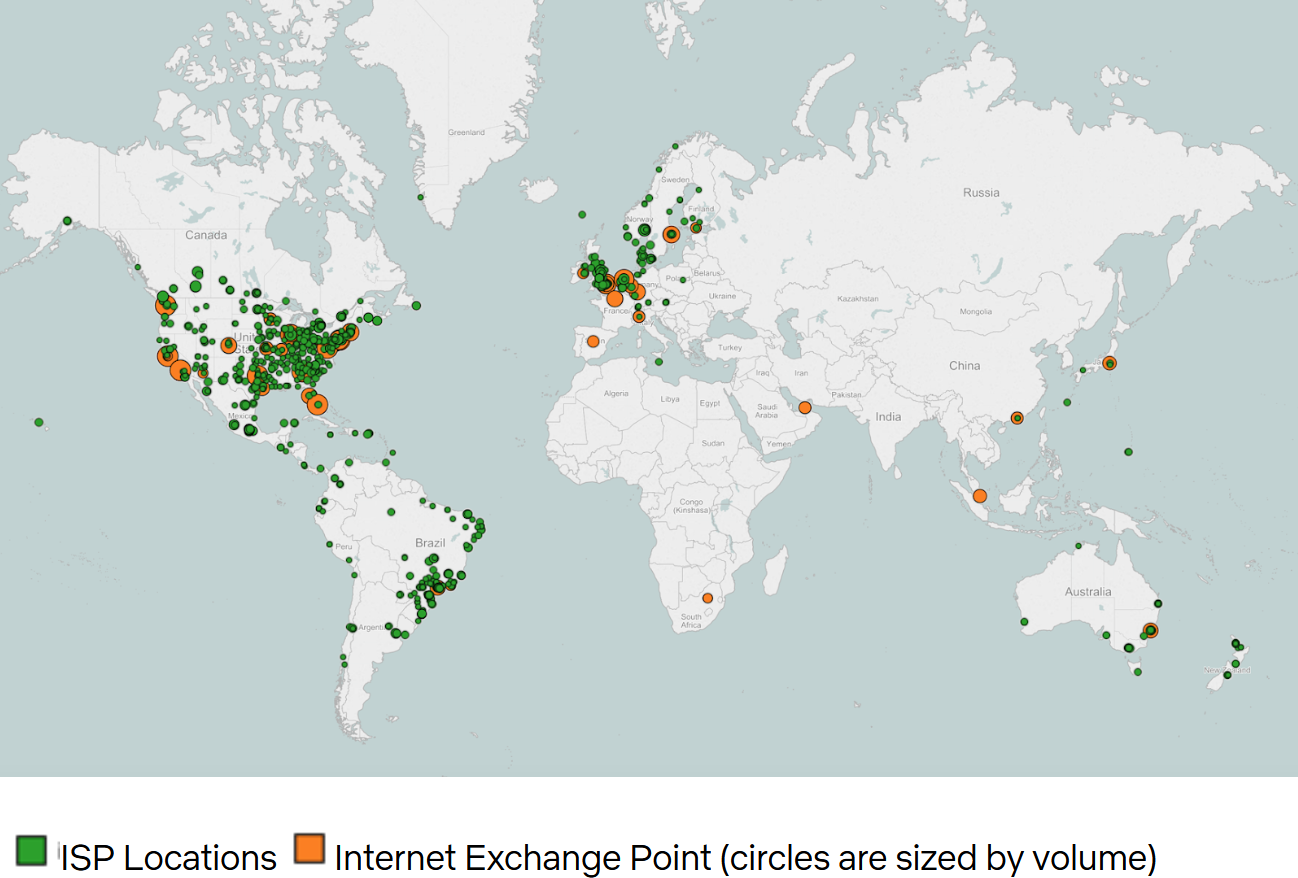
\includegraphics[width=\linewidth]{images/NetflixISP.png}
    \caption[Netflix Open Connect Network as of 2016]{Netflix Open Connect Network as of 2016}\label{fig:netflix-isp}
\end{figure}

\subsection{Content Delivery Mechanism}

Netflix's content delivery strategy involves pre-positioning content on \ac{OCAs} before users request it. This is achieved through advanced predictive algorithms that analyze content popularity, to make sure that the most likely to be watched content is already stored close to where it will be consumed~\parencite{netflix_cloud}. For example, in regions with limited internet capacity, such as Australia, Netflix minimizes the use of undersea cables by pre-loading content onto \ac{OCAs} during off-peak hours, reducing the need for real-time content transmission over these expensive and bandwidth-limited connections.

Netflix also uses consistent hashing to distribute content across multiple servers within a cluster, for balancing workloads and minimizing server churn when the cluster's composition changes~\parencite{netflix_content_distribution}. An example of how this works is the following: Assuming \textit{n} servers, every server ID (\textit{S1} to \textit{Sn}) is hashed 1000 times to generate a reasonably equal distribution of content and also to facilitate fair re-hashing when the cluster changes. Using the uniform consistent hashing approach, then the same weight is assigned to every server.
For heterogeneous server clusters, which consist of servers with varying storage and throughput capacities, Netflix created a 'Heterogeneous Cluster Allocation' algorithm that allocates content based on both the storage and throughput capacities of individual servers, reducing content holes and improving load balance in clusters that were already heterogeneous~\parencite{netflix_content_distribution}.

\subsection{Performance Optimization and Energy Efficiency}

Over the years, Netflix has continuously optimized its \ac{OCAs}, increasing their efficiency by an order of magnitude since the inception of the program. For instance, the throughput of a single server has been increased from 8 Gbps in 2012 to over 90 Gbps in 2016, largely due to improvements in both hardware and software~\parencite{netflix_open_connect}. These advancements have also led to smaller and more power-efficient \ac{OCAs}.
Additionally, Netflix has optimized its content delivery system to handle high levels of encrypted traffic efficiently. Using hardware acceleration and optimizing memory bandwidth usage, Netflix has reached the capability to serve 100 Gbps of encrypted traffic on its modern \ac{OCAs}~\parencite{netflix_content_serving}.

\section{Example: YouTube}

YouTube, launched in 2005, is the world's largest video-sharing platform with over 500 hours of video content uploaded every minute, and approximately 694,000 hours of video content streamed per minute~\parencite{youtube_stats}.

\subsection{General Architecture}

YouTube's infrastructure is built on Google's global network of data centers and \ac{CDN}s: The most popular content for a certain region is cached in global \ac{CDN}s that make sure that there are multiple copies of a video to guarantee quality of service, reliability and closeness to the user while the other videos are stored on separate servers in various locations, mainly in the US~\parencite{youtube_architecture_2}. The platform uses advanced video compression algorithms, such as VP9 and AV1, to optimize bandwidth usage while maintaining high video quality, even at lower bitrates~\parencite{youtube_vpu}. 
In recent years, YouTube has also expanded its feature offering to include livestreaming and 360-degree videos~\parencite{youtube_live}.

The following system design model (see \autoref{fig:youtube-system-design}) will not be explained in detail and is meant to help understand and visualize components referenced in this section~\parencite{youtube_architecture}.

\begin{figure}[htpb]
    \centering
    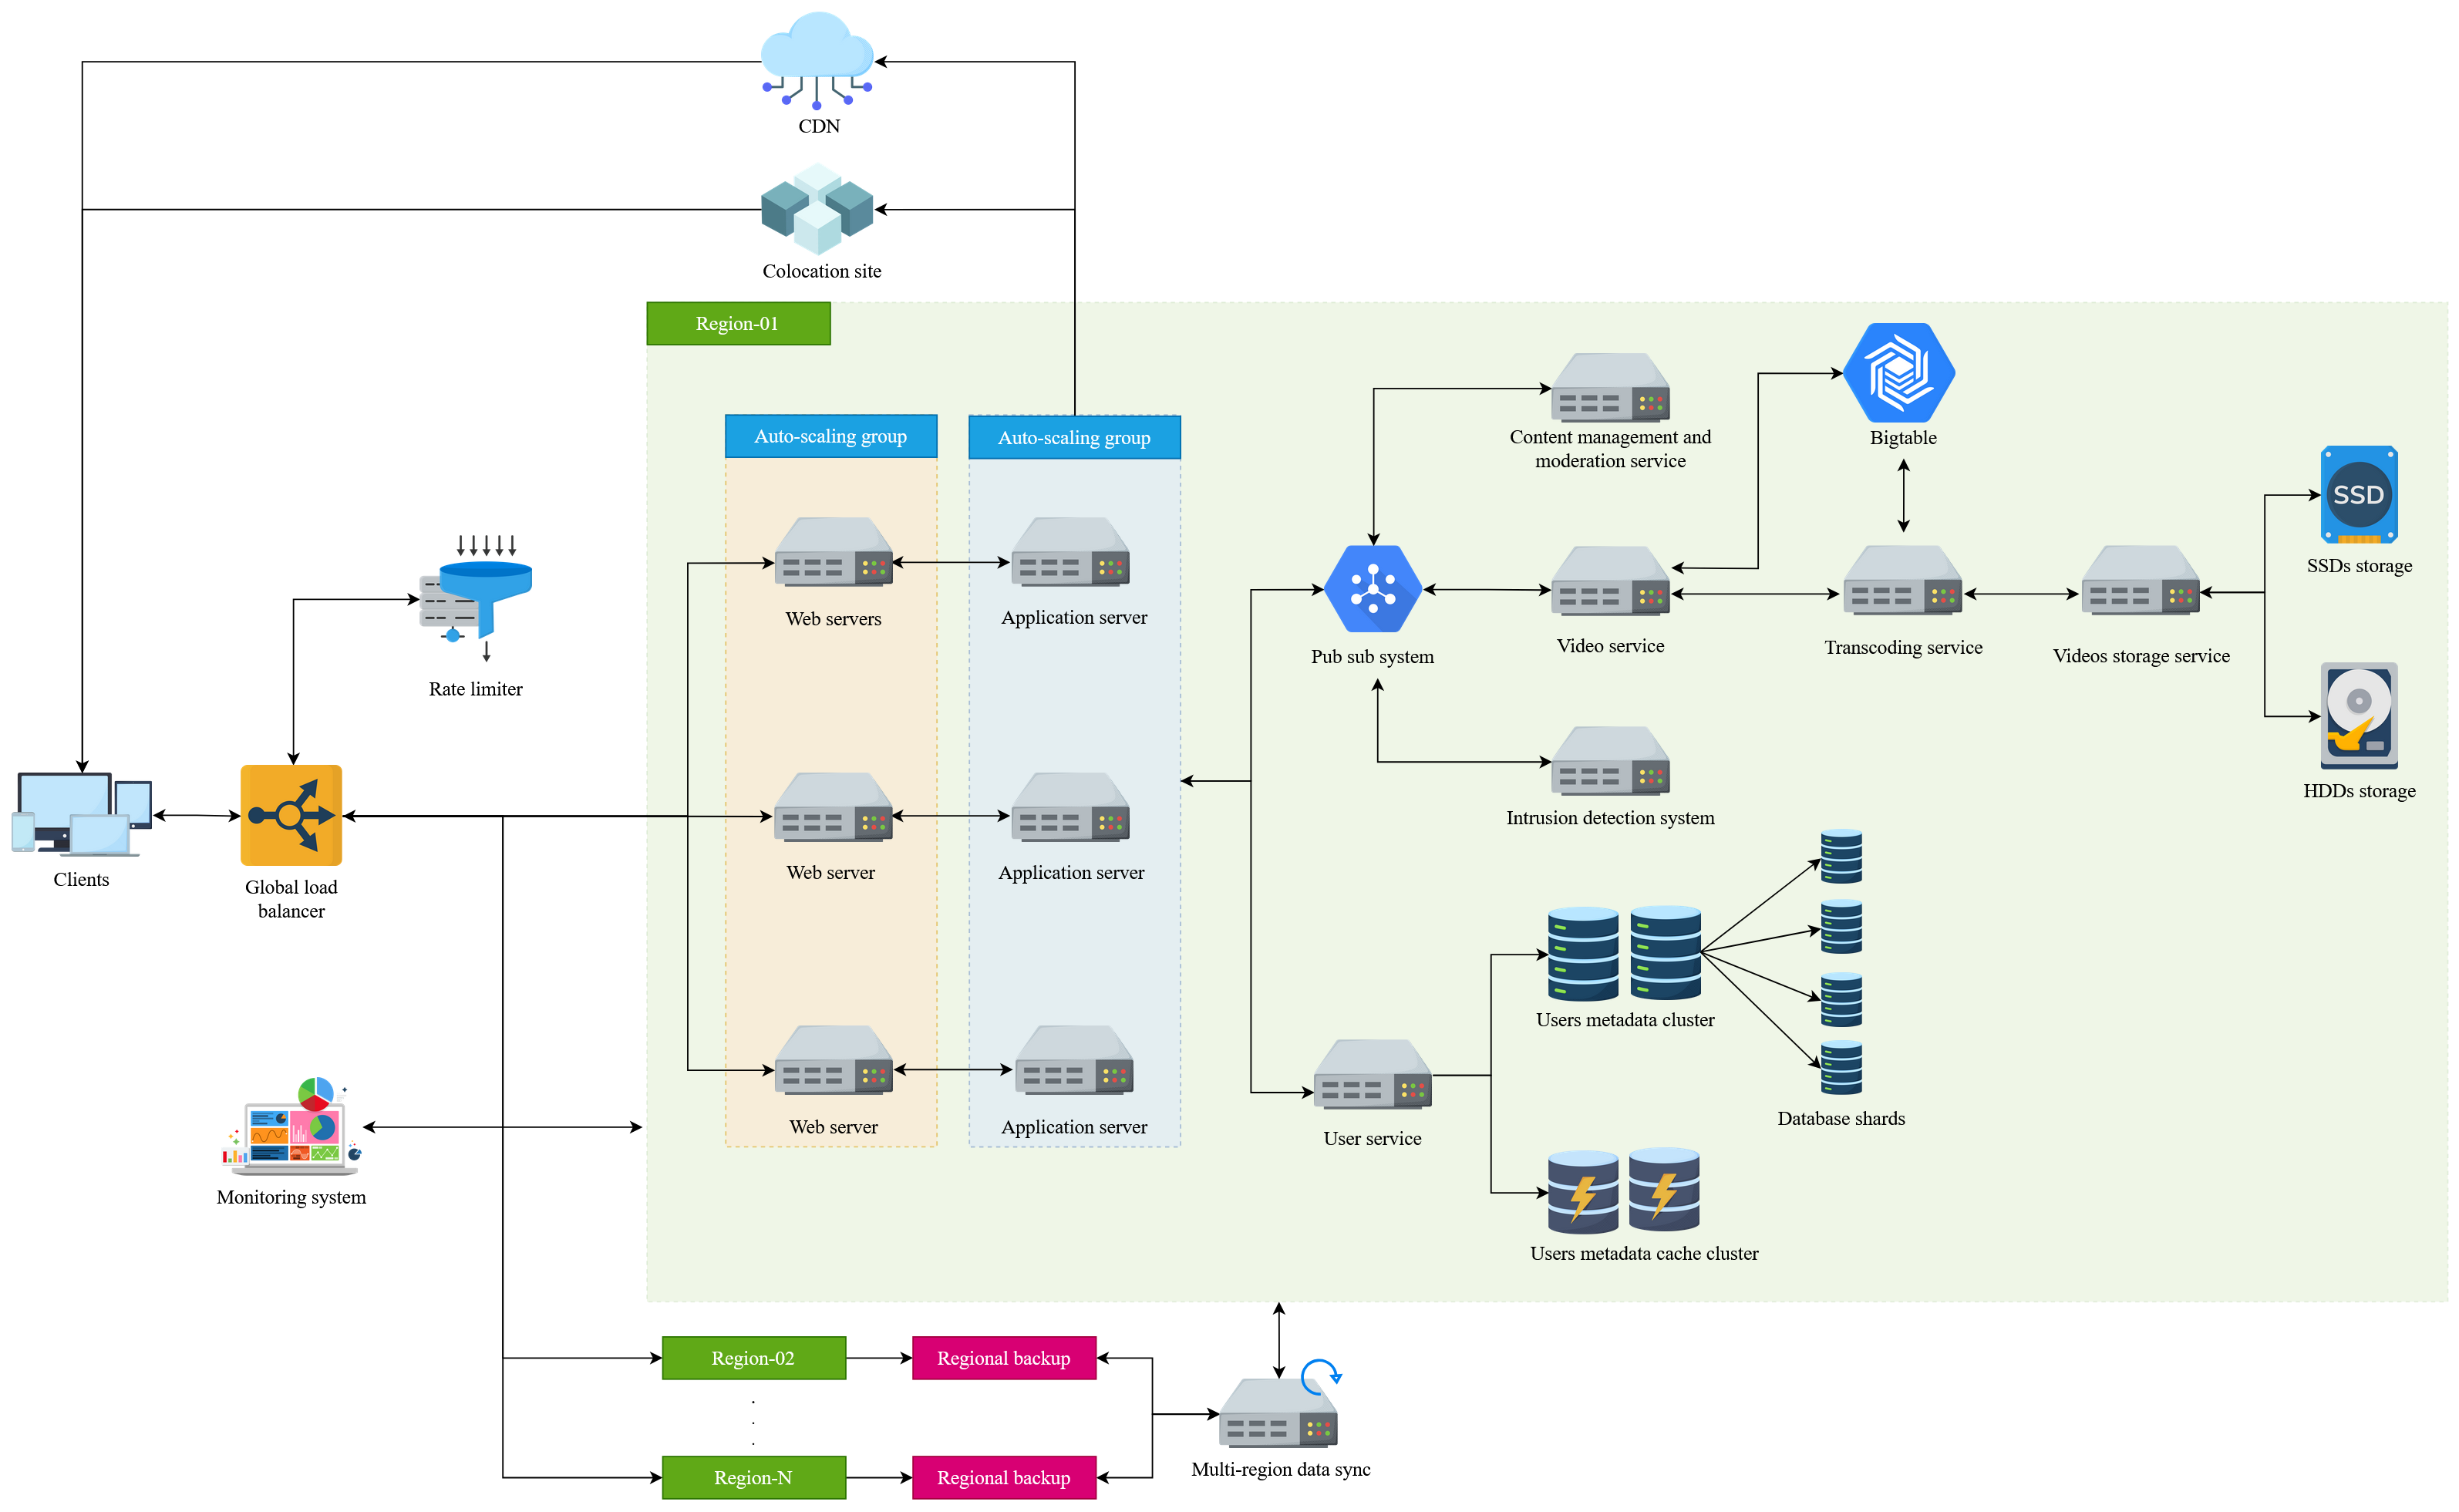
\includegraphics[width=\linewidth]{images/YoutubeSystemDesign.png}
    \caption[YouTube System Design]{YouTube System Design}\label{fig:youtube-system-design}
\end{figure}


\subsection{Scalability Challenges}

While there is not much information on current scalability issues published by YouTube, there are several records of problems that the YouTube team faced up to 2012. These challenges included managing rapid and unpredictable user growth with limited resources, as there was not enough budget to maintain excess machines to handle such growth. Additionally, the integration of new features such as social graphs and recommendation algorithms was especially compute-heavy for the platform. The team also pushed the limits of the hardware and software of that time, encountering limitations like performance bottlenecks in database structures before partitioning~\parencite{youtube_challenges}. As the platform continued to evolve, identifying these bottlenecks became more difficult, as they often were not due to a issue by YouTube itself, but rather by limitations of other libraries and third party software that they used~\parencite{youtube_challenges_2}.

\subsection{Video Acceleration at Scale}

With Moore's Law slowing down, specialized hardware accelerators optimized for large-scale video transcoding are needed to meet demand for video processing. 
In 2021, the YouTube team presented an accelerator called the \ac{VCU} and showed that by scaling it within Google data centers, it achieved 20-33x improved efficiency compared to the previous well-tuned non-accelerated systems (see \autoref{tab:youtube-vcu})~\parencite{youtube_infrastructure}.

\begin{table}[h!]
\centering
\caption{Throughput and Performance Comparison of Systems}\label{tab:youtube-vcu}
\begin{tabular}{|l|cc|cc|}
\hline
\textbf{System}      & \multicolumn{2}{c|}{\textbf{Throughput [Mpix/s]}} & \multicolumn{2}{c|}{\textbf{Perf/TCO}}    \\ \hline
            & \multicolumn{1}{c|}{H.264}       & VP9       & \multicolumn{1}{c|}{H.264} & VP9 \\ \hline
Skylake     & \multicolumn{1}{c|}{714}            & 154           & \multicolumn{1}{c|}{1.0x}      & 1.0x     \\ \hline
4xNvidia T4 & \multicolumn{1}{c|}{2,484}          & --            & \multicolumn{1}{c|}{1.5x}      & --       \\ \hline
8xVCU       & \multicolumn{1}{c|}{5,973}          & 6,122         & \multicolumn{1}{c|}{4.4x}      & \textbf{20.8x}    \\ \hline
20xVCU      & \multicolumn{1}{c|}{14,932}         & 15,306        & \multicolumn{1}{c|}{7.0x}      & \textbf{33.3x}    \\ \hline
\end{tabular}
\end{table}

The core component of the \ac{VCU} system is the encoder core, which serves as a hardware accelerator built for large distributed clusters and works in three stages: 1. \href{https://en.wikipedia.org/wiki/Macroblock}{\textit{Block-based video encoding}} (most memory and bandwidth intensive stage), 2. \href{https://en.wikipedia.org/wiki/Entropy_coding}{\textit{entropy encoding}} and 3. \textit{\href{https://www.kernel.org/doc/html/latest/gpu/afbc.html}{loop filtering and lossless frame buffer compression}}. 
While the \ac{VCU} design optimizes for throughput, system balance and programmability, allowing it to adapt to changing workloads and infrastructure demands, its major challenges are handling multiple resolutions and formats and ensuring system reliability in a large-scale environment~\parencite{youtube_vpu}.
Also, the \ac{VCU} integrates multiple encoder cores and a memory system optimized for data center workloads and can be adjusted dynamically. This hardware-software co-design approach helps efficiently transcode uploaded videos while being flexible for future workloads. The system is highly parallelized, allowing for efficient handling of multi-output transcoding where a single input video is processed into multiple resolutions and formats at the same time~\parencite{youtube_vpu}.

Given the fact that the \ac{VCU} system enables otherwise infeasible VP9 compression, this results in new use cases related to livestreaming (e.g., using VP9 to encode many short (2-second) segments in parallel to increase overall throughput). \blockquote{\textit{As a concrete example, a 2-second 1080p chunk could be encoded in 10 seconds, the encoding system would transcode 5-6 chunks concurrently to achieve the needed throughput of a 1 video-sec/second}}~\parencite{youtube_vpu}.
Currenty, this system is mainly used by YouTube for a wide range of video workloads, including video sharing, live streaming and cloud gaming. 